\documentclass{article}
% \usepackage{sbc-template}
\usepackage{graphicx}
\usepackage[utf8]{inputenc}
\usepackage[T1]{fontenc}
\usepackage{pgfplots}
\usepackage{pgfplotstable} 
\usepackage{titlesec}
\usepackage{lipsum}
\usepackage{authblk}
\usepackage{mathtools}

\begin{document}

\title{Recuperação de Informação - Máquinas de Busca na Web: Trabalho Prático 3}
\author{João Mateus de Freitas Veneroso}
\affil{Departamento de Ciência da Computação da Universidade Federal de Minas Gerais}

\maketitle

\section{Introdução}

Este trabalho descreve a implementação de um sistema de consultas com base no arquivo
invertido criado no trabalho prático 2. O sistema de consulta implementado faz 
consultas ordenadas por meio do modelo de espaço vetorial com a utilização do
anchor text e do page rank para melhoria dos resultados. A interface gráfica do sistema
de consultas foi implementada com o NodeJS e está disponível para consultas na
url visconde.latin.dcc.ufmg.br:8080. A versão mais recente do código pode ser obtida
em: https://github.com/jmfveneroso/inverted-index. Para instruções de compilação e uso, leia
o arquivo README.md. 

\section{Índice invertido}

Esta seção descreve brevemente os detalhes do índice invertido utilizado pelo sistema
de consultas. As páginas foram reindexadas com o mesmo sistema construído no trabalho
prático 2. A coleção completa tem 6.175.317 páginas da web no domínio ".br" ocupando
aproximadamente 477 GB. 

\begin{table}
\centering
\begin{tabular}{ |l|l| }
  \hline
  \multicolumn{2}{|c|}{Etapa de extração} \\
  \hline
  Tamanho da coleção & 477 GB \\
  Número de documentos & 6.175.317 \\
  Número de termos & 9.273.617 \\
  Tamanho do arquivo invertido & 11.20 GB \\
  Tempo de carregamento & 120 s \\
  \hline
\end{tabular}
\caption{Índice invertido}
\label{tab:inverted_index}
\end{table}

As características do arquivo invertido estão descritas na 
tabela \ref{tab:inverted_index}. As \textit{stop words} do inglês e do 
português não foram indexadas. Além disso, somente palavras entre 3 e 30 caracteres
foram consideradas no índice. As listas invertidas de cada termo são comprimidas com
o método Elias-$ \delta $. Além das listas invertidas, o índice contém a norma dos vetores
dos documentos, a frequência do termo na coleção, o page rank dos documentos
e as listas invertidas dos \textit{anchor texts}. O índice está disponível em:
"/mnt/hd0/joao\_test/inverted\_index\_tp3.data" na máquina visconde.latin.

\section{Sistema de consultas}

O sistema de consultas implementado sempre recupera as listas invertidas completas dos termos
procurados e só considera no ranking os documentos que pertencem à interseção das listas invertidas, 
ou seja, os documentos que contém todos os termos procurados. Para palavras que aparecem em muitos documentos, esse
detalhe de implementação pode onerar um pouco a velocidade da máquina de busca. A menor lista 
invertida é recuperada primeiro e, para cada uma das listas invertidas posteriores, apenas os
documentos que já apareceram na primeira lista invertida são mantidos. 

Antes de realizar as buscas, duas estruturas devem ser carregadas em memória principal: 
o dicionário e o mapa de documentos. O dicionário contém todos os termos, a posição das
suas respectivas listas invertidas no arquivo invertido, a posição das suas listas invertidas
de \textit{anchor texts} e a frequência do termo na coleção. O mapa de documentos guarda, 
para cada documento, a id, a url e o page rank. O carregamento destas estruturas 
demora cerca de 120 segundos para o índice descrito na seção anterior. Após o carregamento, as buscas
demoram apenas alguns milisegundos para termos pouco frequentes, mas podem demorar mais para termos
muito frequentes.

O sistema de consultas utiliza três modelos diferentes para realizar o ordenamento dos documentos
encontrados: o modelo vetorial, o modelo de anchor text e o page rank. Cada um destes modelos
possui um peso associado que multiplica o \textit{score} atribuído a cada documento. Estes pesos
servem para ajustar de forma linear a contribuição de cada modelo para o \textit{ranking} final.

\section{Modelo de espaço vetorial}

O modelo de espaço vetorial é o modelo base do nosso sistema de consultas. A medida que as
listas invertidas são analisadas, um acumulador é mantido para cada um dos documentos 
encontrados. Para cada termo, somamos a seguinte expressão ao acumulador:

\begin{equation}
(1 + log(f_{t,d})) \times log(\frac{N}{n_t})
\label{eq:vector}
\end{equation}

onde $ f_{t,d} $ é a frequência do termo no documento, que obtemos na lista invertida do termo, e
$ \frac{N}{n_t} $ é a frequência inversa do termo na coleção, que obtemos no dicionário. Ao
final da análise de todos os documentos, dividimos cada um dos acumuladores pela norma do
seu respectivo documento, que foi salva no índice durante a sua construção. A norma do documento consiste
em somar a equação \ref{eq:vector} para todos os termos da coleção e extrair
a raiz quadrada do resultado. O cálculo dessa soma é trivial após a construção do índice.

\section{Anchor text}

O modelo de \textit{ranking} pelos \textit{anchor texts} funciona com base nos termos
utilizados no texto dos \textit{links} da coleção. Cada termo possui uma lista invertida análoga ao índice principal.
No entanto, essa lista só contém a referência dos documentos apontados pelo 
termo e um contador para saber quantas vezes o termo apareceu apontando cada documento.
\textit{Links} que apontavam documentos fora da coleção foram ignorados. 
O índice de \textit{anchor ranks} para o arquivo invertido descrito na seção 1 ocupa cerca de 2GB.

O \textit{score} atribuído a cada documento é simplesmente o número de vezes que o termo da busca 
foi encontrado em \textit{anchor texts} de \textit{links} que apontavam para um dado documento. 
Para a maioria dos documentos, o \textit{score} será zero. Pois, o volume de texto nos \textit{anchor texts}
é bastante limitado. No entanto, em vários casos de busca, o \textit{anchor text} se mostrou uma 
ferramenta valiosa, já que ele atua como um título para a página apontada.

\section{Page Rank}

O \textit{Page Rank} é uma forma de atribuir relevância aos documentos com base
no conceito de recomendação entre páginas da web, independente dos termos de busca. 
O \textit{Page Rank} foi calculado junto ao índice de \textit{Anchor Texts} 
em uma segunda passagem sobre a coleção após o índice principal já ter sido construído. Para cada \textit{link}
que apontava para um documento dentro da coleção, foi armazenado um ponteiro da origem para o destino,
formando um grafo de recomendação entre os documentos.

Inicialmente, atribuiu-se o valor 1 para cada documento e o algoritmo de cálculo do \textit{Page Rank} foi executado por 300 iterações.
Um alto grau de convergência pode ser alcançado com um número muito menor de iterações, no entanto, já que a coleção é relativamente
pequena, é viável executar um número maior de iterações para alcançar um grau melhor de convergência.

O procedimento executado em cada iteração foi o seguinte: os documentos de origem distribuem seu \textit{score} para os documentos apontados 
pelos seus links. Documentos \textit{sink} (que não contém \textit{links} de saída) têm seu score acumulado e, ao final da iteração,
esse \textit{score} é distribuído entre todos os documentos da coleção. Por conta da distribuição dos \textit{scores}, 
a soma dos \textit{Page Ranks} ao final da iteração é sempre igual ao número de documentos na coleção. No entanto, documentos com
mais "recomendações" acumulam um \textit{score} maior. 

O valor do \textit{Page Rank} é armazenado no mapa de documentos e pode servir para ordenar os documentos por
relevância. No entanto, os resultados são melhores quando ele é usado em associação com outro método como o modelo
de espaço vetorial. Como a ordem de grandeza dos valores artibuídos pelo \textit{Page Rank} acaba sendo muito maior
do que o peso atribuído pelo modelo de espaço vetorial, é necessário usar um fator de normalização, como explicado
na seção 2. O \textit{Page Rank} se mostrou um sinal ainda mais eficiente quando utilizado
em combinação com o índice de \textit{anchor texts}.

\section{Servidor e interface gráfica}

O servidor da máquina de busca foi implementado no \textit{NodeJS}, um \textit{runtime environment} 
que executa \textit{Javascript} do lado do servidor. Um módulo do \textit{node-gyp} foi construído
para transformar a máquina de busca (C++) em uma biblioteca do \textit{Javascript}. O servidor
utiliza o \textit{framework} Express para responder às requisições http e a linguagem de marcação 
Jade para construir a interface gráfica. 

O servidor responde requisições nas rotas:

\subsubsection{GET /}

\begin{figure}
\centering
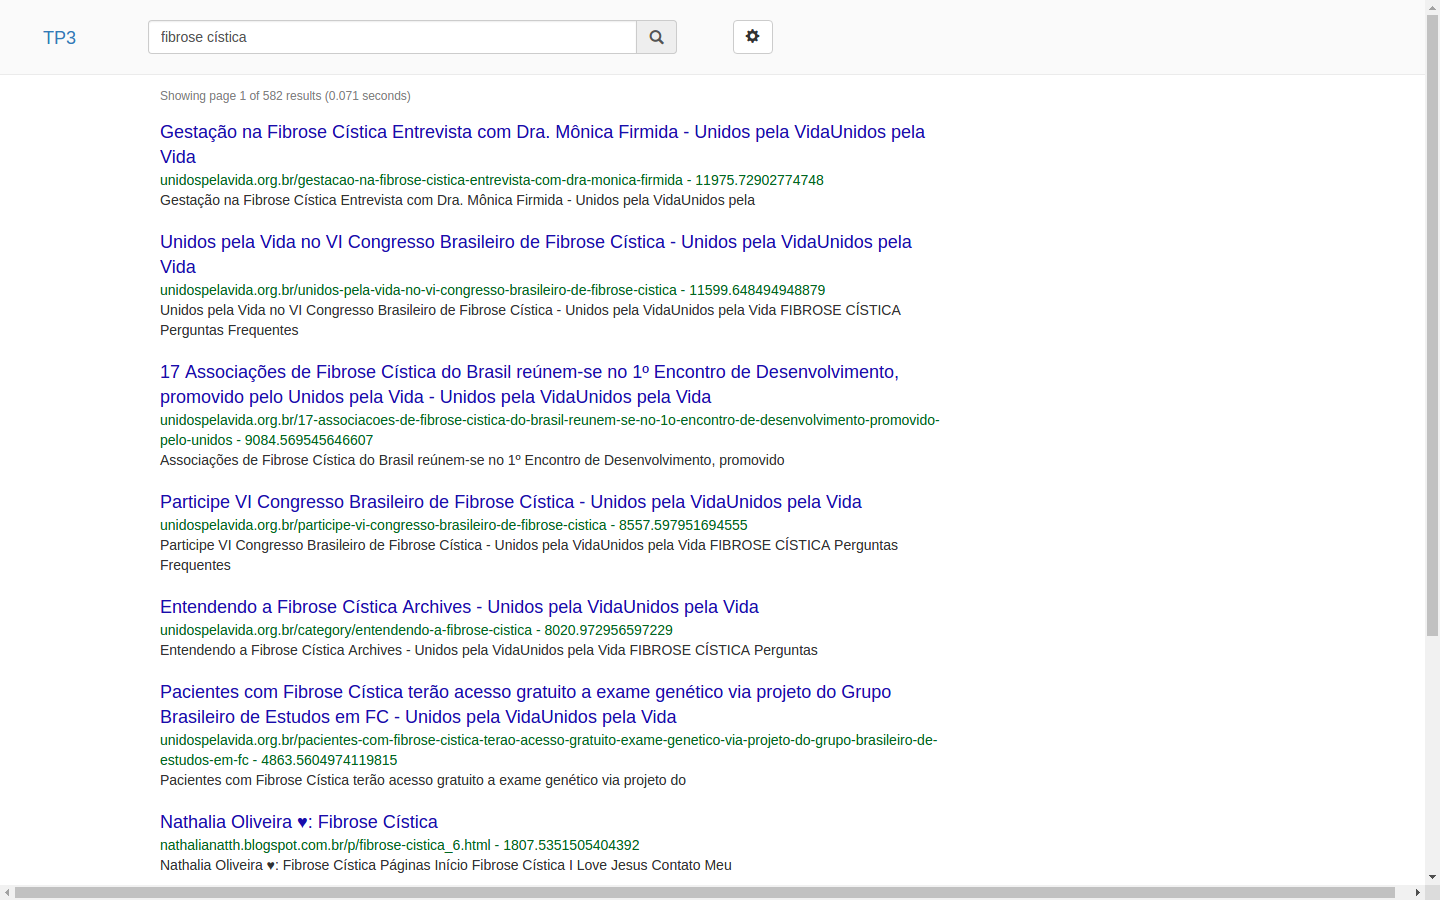
\includegraphics[width=\linewidth]{page_1.png}
\caption{Página inicial com a consulta: "fibrose cística"} 
\label{fig:page_1}
\end{figure}

\begin{figure}
\centering
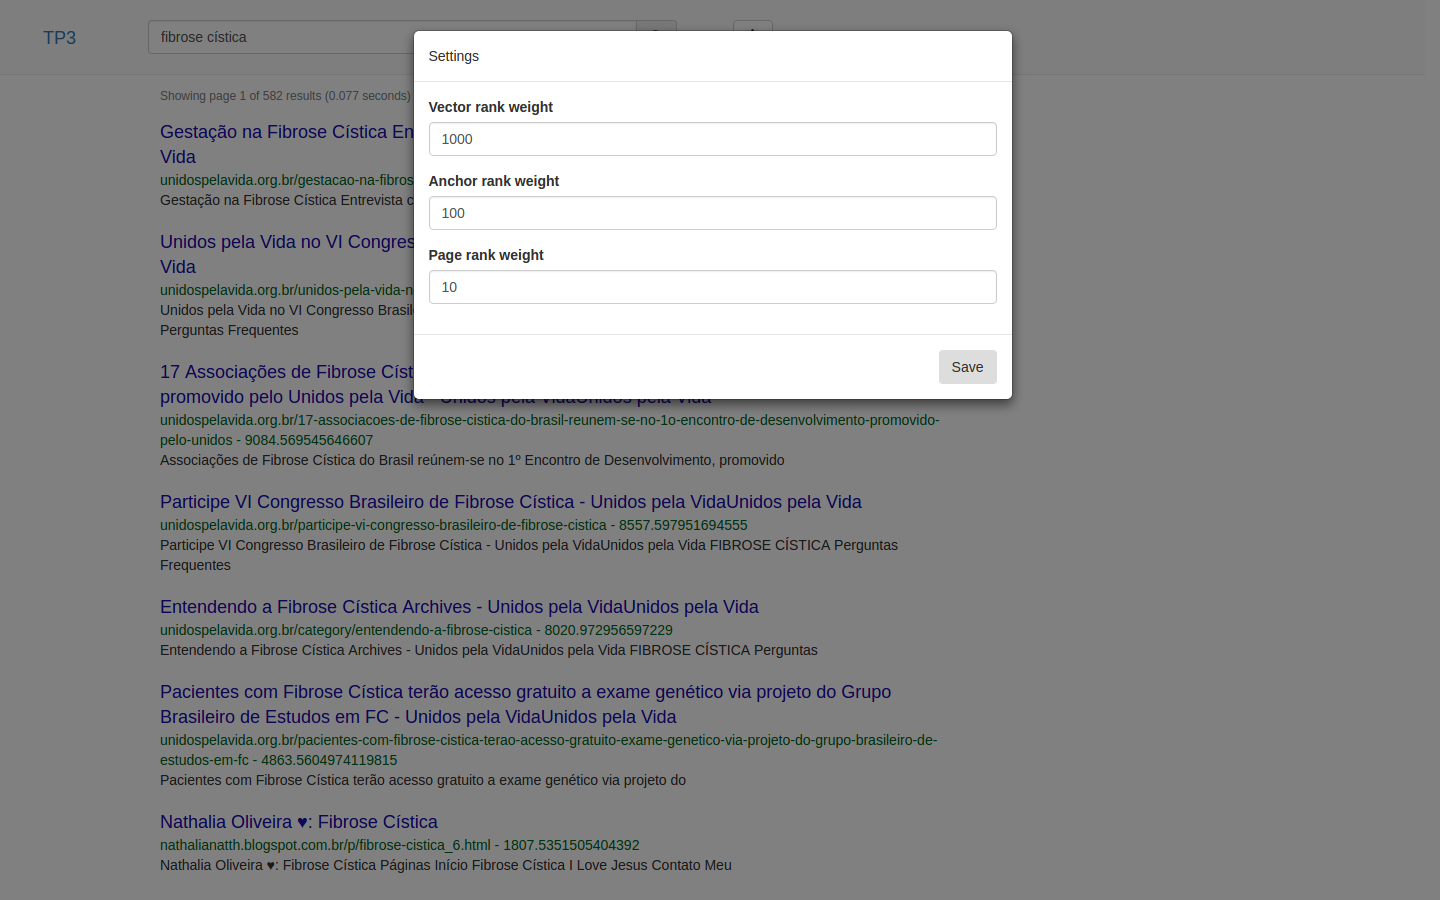
\includegraphics[width=\linewidth]{page_1_modal.png}
\caption{Modal de ajuste dos pesos relativos dos modelos de ordenamento} 
\label{fig:page_1_modal}
\end{figure}

\begin{figure}
\centering
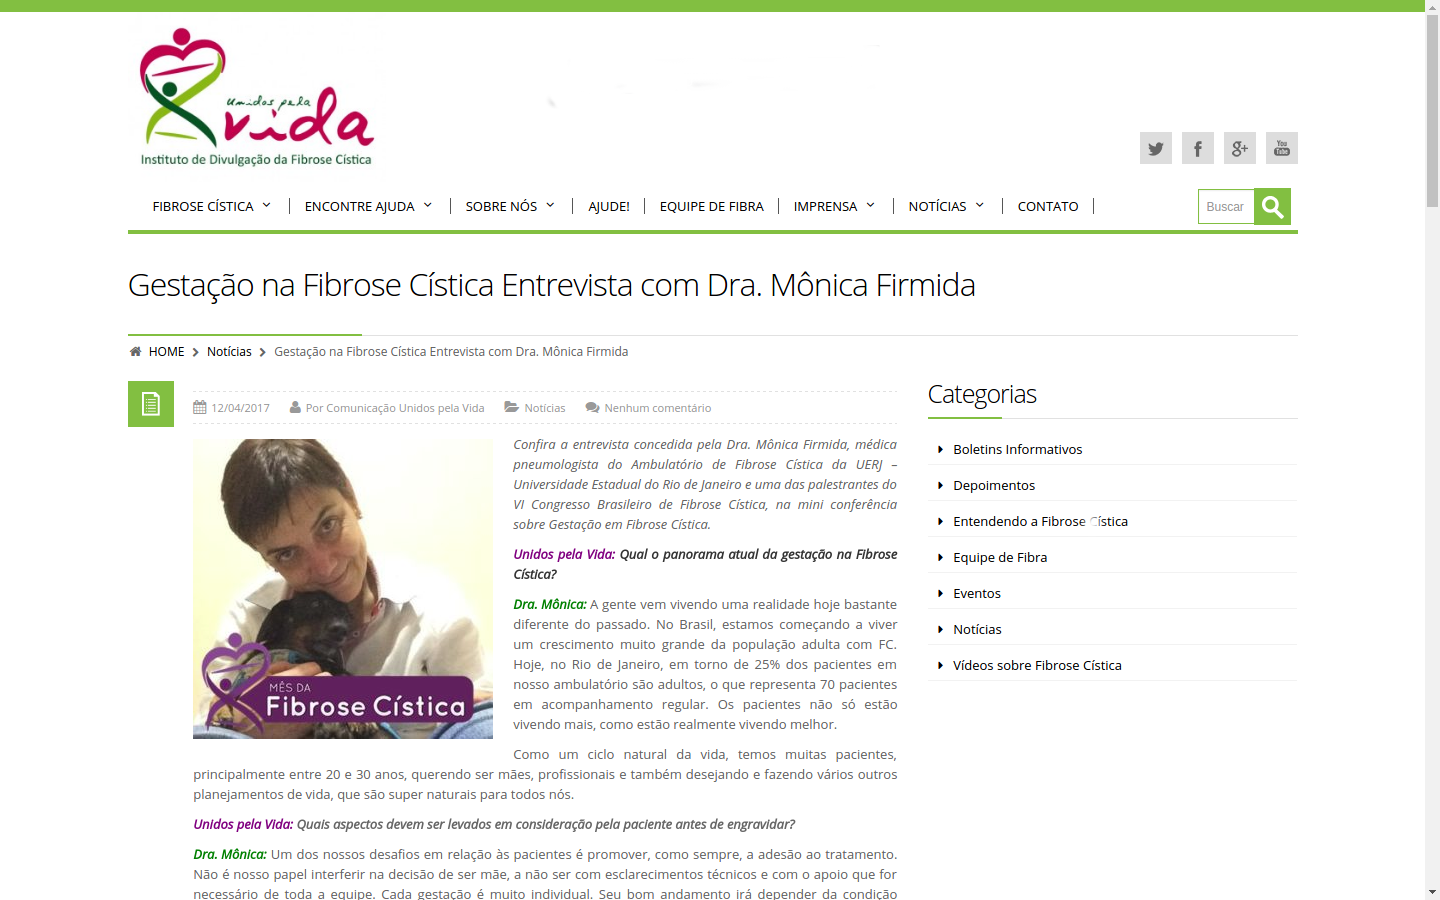
\includegraphics[width=\linewidth]{doc.png}
\caption{Exemplo de conteúdo de página} 
\label{fig:doc}
\end{figure}

A página inicial conta com uma caixa de texto onde o usuário pode fazer consultas. A figura \ref{fig:page_1}
mostra um exemplo de consulta. 
Um ícone à esquerda da caixa de consultas abre um modal onde os pesos relativos dos modelos de \textit{ranking}
podem ser ajustados (basta colocar zero no campo para desativar um modelo), como mostrado na figura
\ref{fig:page_1_modal}. A página só mostra 
10 resultados. Para navegar pelas próximas páginas de resultados é necessário clicar nos botões
"Previous Page" e "Next Page" na parte de baixo da página.
Cada resultado mostra o título da página (extraído da tag <title> no html), a url da página 
seguida do \textit{score} e um pequeno trecho onde os termos buscados
ocorrem no documento.

Parâmetros: 
\begin{itemize}
  \item q = consulta
  \item vector = peso do modelo de espaço vetorial (padrão = 1000)
  \item anchor = peso do modelo de anchor texts (padrão = 100)
  \item pagerank = peso do page rank (padrão = 10)
  \item page = página atual da consulta (padrão = 1)
\end{itemize}

\subsubsection{GET /doc}
A rota /doc mostra o conteúdo de um documento. Como o html extraído pelo crawler pode conter links para
arquivos CSS e Javascript que não existem mais, a apresentação da página pode ficar prejudicada. A 
figura \ref{fig:doc} mostra o conteúdo da primeira página retornada pela consulta "fibrose cística". 

Parâmetros: 
\begin{itemize}
  \item id = id do documento
\end{itemize}

\section{Experimentos}

\subsection{vivo}
\subsection{itau}
\subsection{uol}
\subsection{g1}

Não há resultados para essa pesquisa, porque o índice desconsidera
palavras com menos de três caracteres.

\subsection{banco brasil}
\subsection{belo horizonte}
\subsection{folha}
\subsection{decolar}
\subsection{Pokemon GO}
\subsection{Jogos Olímpicos Rio 2016}
\subsection{Big Brother Brasil}
\subsection{Tabela do Brasileirão}
\subsection{Enem}
\subsection{Sisu}
\subsection{iPhone 7}
\subsection{Ana Hickmann}
\subsection{Donald Trump}
\subsection{Renato Aragão}
\subsection{Camila Pitanga}
\subsection{Diego Hypólito}
\subsection{Logan}
\subsection{A bela e a fera}
\subsection{Power Rangers}
\subsection{o que é crush}
\subsection{o que é amor}
\subsection{o que é filosofia}
\subsection{como fazer crepioca}
\subsection{como fazer bolo}
\subsection{como fazer bolo de pote}
\subsection{por que o feijão esta tão caro}

\section{Conclusão}

O objetivo do trabalho prático 3 era implementar um sistema de consultas e uma interface gráfica. O resultado
está disponível em visconde.latin.dcc.ufmg.br:8080 (só funciona na porta 8080). Os sinais do
\textit{anchor text} e do \textit{page rank} mostraram uma melhora considerável na efetividade
das consultas, no entanto, o resultado final ainda mostrou um desempenho aquém do desejável em
um cenário de busca realista.

\end{document}
